\section{Fluid Theory}
\begin{frame}{Fluid Equations - Moments of $f$}
    From the distribution function $f(\mathbf{x},\mathbf{v}',t)$, we can get its moments by multiplying it with functions of $\mathbf{v}'$ and integrate them.
    \begin{equation}
        \begin{aligned}
            n          & = \int f(\mathbf{x},\mathbf{v}',t)\dd{\mathbf{v}'}                                \\
            \mathbf{v} & = \frac{1}{n}\int f(\mathbf{x},\mathbf{v}',t)\mathbf{v}'\dd{\mathbf{v}'}          \\
            \mathbf{P} & = m\int f(\mathbf{x},\mathbf{v}',t)(\mathbf{v'-v})(\mathbf{v'-v})\dd{\mathbf{v}'}
        \end{aligned}
        \label{eq:distribution-moments}
    \end{equation}
    where $\mathbf{P}$ is pressure tensor. For spatial homogeneous distribution function, the scalar pressure is given by
    \begin{equation}
        p = \frac{1}{3}m\int f(\mathbf{x},\mathbf{v}',t)(\mathbf{v'-v})^2\dd{\mathbf{v}'}
        \label{eq:scalar-pressure}
    \end{equation}
\end{frame}

\begin{frame}{Fluid Equations - Equations of Motion}
    Apply the same procedure in previous slide to Fokker-Planck Equation, Eq.(\ref{eq:fokker-planck-equation}), we are able to get equations of motions,
    \begin{itemize}
        \item Continuity Equation:
              \begin{equation}
                  \pdv{n}{t} + \div(n\mathbf{v}) = 0
                  \label{eq:conservation-of-density}
              \end{equation}
        \item Momentum Equation:
              \begin{equation}
                  nm\left( \pdv{\mathbf{v}}{t} + \mathbf{v}\cdot\grad\mathbf{v} \right) = -\div\mathbf{P} + nZe(\mathbf{E+v\times B}) + \mathbf{R}
                  \label{eq:conservation-of-momentum}
              \end{equation}
              where $\mathbf{R} = \int m\mathbf{v'}\left(\pdv{f}{t}\right)_c\dd{\mathbf{v'}}$.
    \end{itemize}
    We can continue this process and get more equations of higher moments $f$, e.g. heat equation.

    Fluid equations are only valid when the mean free path is small enough compare to the macroscopic scale. So not valid for high temperature plasma.
\end{frame}

\begin{frame}{Magnetohydrodynamics - Ideal MHD}
    To close the set of fluid equations, we need an extra equation of state (EOS), the adiabatic equation,
    \begin{equation}
        \dv{t}\,(p\rho^{-\gamma}) = 0
        \label{eq:adibatic-equation}
    \end{equation}

    Using the vacuum Maxwell's equations, and fluid equations together with EOS, we have the so-called ideal MHD equations,
    \begin{table}
        \centering
        \caption{The equations of ideal mhd.}
        \begin{tabular}{ll}
            \hline
            $\pdv{\rho}{t}           = -\rho\div\mathbf{v}           $ & $\mu_0\mathbf{j} = \curl\mathbf{B}$           \\
            $\rho\dv{\mathbf{v}}{t}  = \mathbf{j\times B} - \grad{p} $ & $\pdv{\mathbf{B}}{t}     = - \curl\mathbf{E}$ \\
            $\dv{p}{t}               = -\gamma p\div\mathbf{v}       $ & $\mathbf{E + v\times B}  = 0$                 \\
            \hline
        \end{tabular}
        \label{table:ideal-mhd}
    \end{table}
\end{frame}

\begin{frame}{Magnetohydrodynamics - Resistive MHD}
    To get resistive MHD equations, we only need to replace the adiabatic equation to
    \begin{equation}
        \dv{t}\,\left(\frac{p}{\gamma-1}\right) = \frac{\gamma}{\gamma-1}p\div\mathbf{v} + \eta j^2
        \label{eq:resistive-adibatic-equation}
    \end{equation}

    And the $\mathbf{E+v\times B} = 0$ to Ohm's law $\mathbf{E+v\times B} = \eta\mathbf{j}$
\end{frame}

\begin{frame}{Plasma Diamagnetism}
    \begin{itemize}
        \item Plasma is always diamagnetic due to the Larmor motions of particles weakens the applied magnetic field, see.
        \item The total diamagnetic current is given by $\mathbf{j = j_s + j_d}$, where $\mathbf{j_s} = \mathbf{b}\times\grad(p/B)$ is the current induced by particle gyration, and $\mathbf{j_d} = \mathbf{b}\times (p/B^2)\grad B$ is the drift current.
    \end{itemize}
\end{frame}

\begin{frame}{Plasma Diamagnetism - Figures}
    \begin{figure}
        \begin{subfigure}[b]{0.4\textwidth}
            \centering
            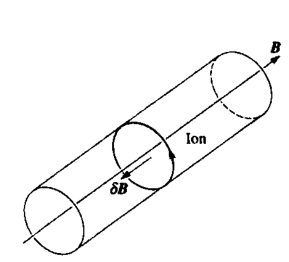
\includegraphics[width=0.7\textwidth]{figures/plasma-diamagnetism.png}
            \caption{Ions with a given velocity having Larmor orbits on a cylinder produce a magnetic field $\delta B$ inside the cylinder, this field being in the opposite direction to the total magnetic field B.}
            \label{fig:plasma-diamagnetism}
        \end{subfigure}%
        \begin{subfigure}[b]{0.4\textwidth}
            \centering
            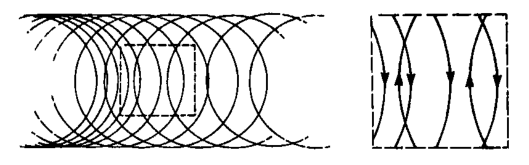
\includegraphics[width=\textwidth]{figures/diamagnetic-current.png}
            \caption{Showing how a density gradient of stationary orbits give rise to a current. The current arises through a local imbalance of upward and downward moving particles as illustrated in the enlarged secion.}
            \label{fig:diamagnetic-current}
        \end{subfigure}
    \end{figure}
\end{frame}

\begin{frame}{Braginskii Equations}
    \begin{itemize}
        \item Coulomb collisions do not change the number of particles.
        \item Friction force: $\mathbf{R_u} = - (m_en/\tau_e)(0.51u_\parallel + u_\perp) = ne(\eta_\parallel j_\parallel + \eta_\perp j_\perp)$, where $\mathbf{u=v_e-v_i}$
        \item Thermal force: $\mathbf{R_T} = -0.71n\grad_\parallel T_e - \frac{3}{2}\frac{n}{\abs{\omega_{ce}\tau_e}\mathbf{b}\times\grad T_e}$
        \item Ion heating: $Q_i = \frac{3m_e}{m_i}\frac{n}{\tau_e}(T_e-T_i)$.
        \item Electron heating: $Q_e = -\mathbf{R\cdot u} - Q_i = \eta_\parallel j_\parallel^2 + \eta_\perp j_\perp^2 + \frac{1}{ne}\mathbf{j\cdot R_T} + \frac{3m_e}{m_i}\frac{n}{\tau_e}(T_i-T_e)$
    \end{itemize}
    Some interesting things,
    \begin{itemize}
        \item The ratio of parallel to perpendicular thermal conductivity is $(\omega_{c}\tau)^2$. It is $10^{13}$ for electrons and $10^{16}$ for ions.
        \item In parallel direction, electron thermal conductivity is larger than that of ions by a factor $\sim (m_i/m_e)^2$ because of their long collision time.
        \item In perpendicular direction, the relationship is reversed because of the larger ion Larmor radius.
        \item The ohm heating $\eta j^2$ appears only in electrons because they only transfer $\sim m_e/m_i$ of energy to ions.
    \end{itemize}
\end{frame}

\begin{frame}{Plasma Waves - Dispersion Relations}
    \begin{itemize}
        \item Transverse EM wave:
              \begin{equation}
                  \omega^2 = k^2c^2 + \omega_p^2
                  \label{eq:transverse-wave}
              \end{equation}
        \item Sound wave:
              \begin{equation}
                  \omega^2 = k^2c_s^2,\;\; c_s^2 = \gamma\frac{p_i + p_e}{nm_i}
                  \label{eq:}
              \end{equation}
        \item Shear Alfven wave, see Fig:
              \begin{equation}
                  \omega = k_xv_A,\;\; v_A = B_0/\sqrt{\mu_0\rho}
                  \label{eq:shear-alfven-wave}
              \end{equation}
        \item Magnetosonic waves:
              \begin{equation}
                  \frac{\omega^2}{k^2} = \frac{1}{2} \{ c_s^2 + v_A^2 \pm [(c_s^2+v_A^2)^2 - 4c_s^2v_A^2\cos^2\theta]^{1/2} \}
                  \label{eq:magnetosonic-wave}
              \end{equation}
              The fast magnetosonic wave given by choosing the $+$ sign, and the slow magnetosonic wave given by choosing the $-$ sign.
    \end{itemize}
\end{frame}

\begin{frame}{Plasma Wave - Alfven Wave}
    \begin{figure}
        \centering
        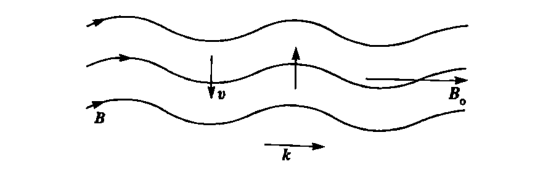
\includegraphics[width=0.6\textwidth]{figures/simple-alfven-wave.png}
        \caption{Simple Alfven wave with $k\parallel B_0$. The fluid velocity oscillates in the plane of the figure.}
        \label{fig:simple-alfven-wave}
    \end{figure}
    \begin{figure}
        \centering
        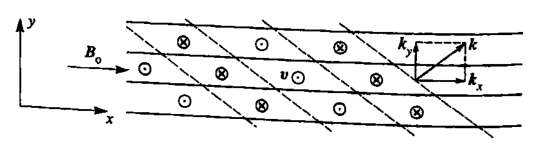
\includegraphics[width=0.6\textwidth]{figures/shear-alfven-wave.png}
        \caption{General shear Alfven wave. $B_0$ and $k$ lie in the plane of the figure and the velocity oscillation is perpendicular to this plane. The wave propagates along $x$ with the Alfven velocity $v_A$.}
        \label{fig:shear-alfven-wave}
    \end{figure}
\end{frame}

\begin{frame}{Plasma Wave - Magnetosonic Wave}
    \begin{figure}
        \centering
        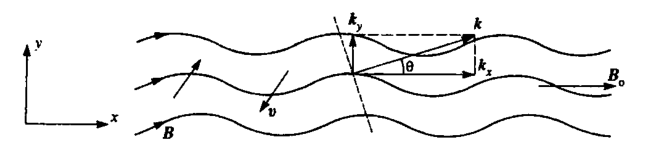
\includegraphics[width=0.7\textwidth]{figures/magnetosonic-wave.png}
        \caption{The magnetosonic wave has velocity oscillations in the plane containing $B_0$ and $k$.}
        \label{fig:magnetosonic-wave}
    \end{figure}
    \begin{figure}
        \centering
        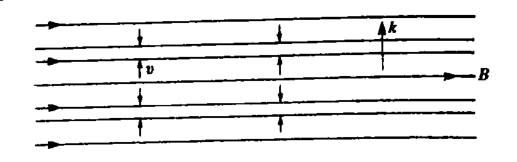
\includegraphics[width=0.6\textwidth]{figures/magnetosonic-wave-fast.png}
        \caption{The fast magnetosonic with $k\perp B_0$. The oscillations involve compression of both the fluid and the magnetic field.}
        \label{fig:magnetosonic-wave-fast}
    \end{figure}
\end{frame}